% ==============================================================================
% CHƯƠNG 2: HIỂU DỮ LIỆU VÀ EDA (DATA UNDERSTANDING & EDA)
% ==============================================================================

\chapter{Hiểu Dữ Liệu và Khám Phá EDA (Data Understanding)}
\label{chap:data_understanding}

\section{Nguồn Thu Thập Dữ Liệu Nghiên Cứu Khoa Học}

Để xây dựng một kho dữ liệu học thuật quy mô lớn, có tính cập nhật thời sự và bao quát cả các công trình nền tảng lịch sử, hệ thống khai thác dữ liệu từ sáu nguồn học thuật uy tín:

\begin{enumerate}[label=\textbf{\arabic*.}]
  \item \textbf{arXiv RSS Feeds \& OAI-PMH API}: Nguồn dữ liệu chủ lực cung cấp các công trình nghiên cứu mới nhất thuộc các nhóm ngành Khoa học Máy tính (Computer Science) và Thống kê (Statistics). Hệ thống sử dụng giao thức OAI-PMH với cơ chế phân trang tự động \texttt{resumptionToken} để thu thập hàng chục nghìn bài báo kèm siêu dữ liệu chuẩn Dublin Core.
  \item \textbf{arXiv HTML5 / ar5iv Project}: Nguồn văn bản giàu định dạng (rich document source) do dự án ar5iv (hợp tác cùng nhóm LaTeXML tại Viện Tiêu chuẩn và Kỹ thuật Quốc gia Hoa Kỳ - NIST) chuyển đổi trực tiếp từ mã nguồn TeX của tác giả sang định dạng HTML5 ngữ nghĩa. Nguồn này hỗ trợ bóc tách LaTeX khi HTML có annotation hoặc alttext phù hợp; mức độ bảo toàn phụ thuộc chất lượng tài liệu nguồn.
  \item \textbf{OpenAlex \& Semantic Scholar}: Nguồn bổ trợ cung cấp đồ thị trích dẫn học thuật toàn cầu, chỉ số ảnh hưởng của tác giả, và các công trình kinh điển (Foundation Papers như \textit{Attention Is All You Need}, \textit{ResNet}, \textit{BERT}, \textit{Adam Optimizer}) giúp xây dựng mạng lưới trích dẫn xương sống.
  \item \textbf{OpenReview.net}: Thu thập các bài báo hội nghị (ICLR, NeurIPS) và có module thu thập review. Schema Silver papers/chunks hiện chưa chứng minh việc đưa toàn bộ review, score và rebuttal vào ngữ cảnh RAG.
  \item \textbf{Computer Vision Foundation (CVF) Open Access}: Bổ sung các bài báo hội nghị chuyên ngành Thị giác máy tính đỉnh cao như CVPR 2024.
  \item \textbf{Zenodo Open Repository}: Lưu trữ các tập dữ liệu thực nghiệm và tài liệu bổ trợ khoa học.
\end{enumerate}

\section{Cấu Trúc Bản Ghi và Siêu Dữ Liệu Học Thuật (Silver Schema)}

Dữ liệu sau khi thu thập từ các nguồn thô được chuẩn hóa và tổ chức thành các bảng Parquet dạng cột trong tầng Silver. Mỗi bản ghi tài liệu khoa học tuân thủ nghiêm ngặt cấu trúc lược đồ (schema) gồm các trường thông tin sau:

\begin{itemize}
  \item \texttt{paper\_id} (String): Mã định danh duy nhất của bài báo (ví dụ: \texttt{2401.13216}, \texttt{2310.01407}).
  \item \texttt{title} (String): Tiêu đề bài báo đã được làm sạch khoảng trắng và chuẩn hóa ký tự Unicode.
  \item \texttt{abstract} (String): Tóm tắt nội dung bài báo.
  \item \texttt{authors} (List[String]): Danh sách tên đầy đủ của tất cả các tác giả tham gia công trình.
  \item \texttt{primary\_category} (String): Phân ngành chính theo phân loại của arXiv (ví dụ: \texttt{cs.LG}, \texttt{cs.CV}).
  \item \texttt{categories} (List[String]): Danh sách tất cả các nhãn chuyên ngành mà tác giả đăng ký (thể hiện tính liên ngành).
  \item \texttt{published\_date} (String): Ngày công bố chính thức hoặc ngày cập nhật phiên bản mới nhất.
  \item \texttt{total\_sections} (Integer): Tổng số mục/chương có cấu trúc được bóc tách từ bài báo.
  \item \texttt{total\_math\_count} (Integer): Tổng số lượng công thức toán học dạng LaTeX (công thức inline và display).
  \item \texttt{total\_words} (Integer): Tổng số lượng từ vựng của toàn văn bài báo.
  \item \texttt{clean\_full\_text} (String): Toàn văn bài báo đã được lọc bỏ các thẻ HTML rác và giữ lại cấu trúc ngữ nghĩa.
  \item \texttt{sections\_json} (JSON String): Cấu trúc phân đoạn chi tiết, bao gồm tiêu đề mục (\texttt{section\_title}), loại mục (\texttt{section\_type}: abstract, introduction, methodology, experiments, conclusion), và nội dung chi tiết.
  \item \texttt{abstract\_hash} (String): SHA-256 của abstract chuẩn hóa (hoặc title nếu abstract trống), phục vụ khử trùng lặp. Các trường nguồn gồm \texttt{source}, \texttt{tier}, \texttt{content\_origin}; thời điểm gồm \texttt{crawled\_at}, \texttt{transformed\_at}.
\end{itemize}

\section{Thống Kê Mô Tả Toàn Cảnh Hồ Dữ Liệu (Descriptive Statistics)}

Snapshot local \path{data/gold/mining/eda_summary.json}, được manifest ngày 04/10/2026 tham chiếu, ghi nhận \textbf{10,000 bài}, trong đó \textbf{9,015 bài làm giàu HTML} ($90.15\%$), \textbf{47,782,707 từ} và \textbf{2,220,938 công thức}. Trung bình có 4,778.27 từ và 222.09 công thức/bài. Ngày công bố trong snapshot từ 28/12/2005 đến 21/02/2024.

Đây là snapshot lịch sử lưu trong repository, không phải phép đo trực tiếp MinIO/Qdrant hiện tại. Báo cáo không gộp thêm số liệu từ các đợt thu thập chưa có artifact đối chiếu.

Bảng~\ref{tab:eda_categories} trình bày phân bố chi tiết số lượng bài báo, công thức toán và độ dài trung bình theo từng chuyên ngành khoa học.

\begin{table}[htbp]
\centering
\small
\caption[Phân bố chuyên ngành trong snapshot 10,000 bài]{Phân bố chuyên ngành trong snapshot 10,000 bài}
\label{tab:eda_categories}
\begin{tabularx}{\textwidth}{|p{2.3cm}|L|L|L|L|L|}
\hline
\textbf{Ngành} & \textbf{Số bài} & \textbf{Tỷ lệ} & \textbf{Công thức} & \textbf{CT/bài} & \textbf{Từ TB/bài} \\
\hline
cs.LG & 2,380 & 23.80\% & 886,955 & 372.7 & 5,099.7 \\
\hline
cs.CV & 2,271 & 22.71\% & 308,487 & 135.8 & 4,432.7 \\
\hline
cs.CL & 1,467 & 14.67\% & 149,869 & 102.2 & 4,315.5 \\
\hline
cs.RO & 682 & 6.82\% & 101,023 & 148.1 & 4,636.6 \\
\hline
cs.AI & 453 & 4.53\% & 94,302 & 208.2 & 5,383.9 \\
\hline
eess.IV & 294 & 2.94\% & 32,010 & 108.9 & 3,559.7 \\
\hline
cs.IR & 253 & 2.53\% & 32,976 & 130.3 & 4,706.7 \\
\hline
stat.ML & 222 & 2.22\% & 148,723 & 669.9 & 6,119.4 \\
\hline
Còn lại (suy từ tổng) & 1,978 & 19.78\% & 466,593 & 235.9 & -- \\
\hline
Toàn snapshot & 10,000 & 100.00\% & 2,220,938 & 222.1 & 4,778.3 \\
\hline
\end{tabularx}
\ReportNote{Nguồn: Thống kê mô tả phân bố chuyên ngành chính trên tập dữ liệu chuẩn 10,000 bài báo từ \path{data/gold/mining/eda_summary.json}.}
\end{table}


\begin{figure}[htbp]
  \centering
  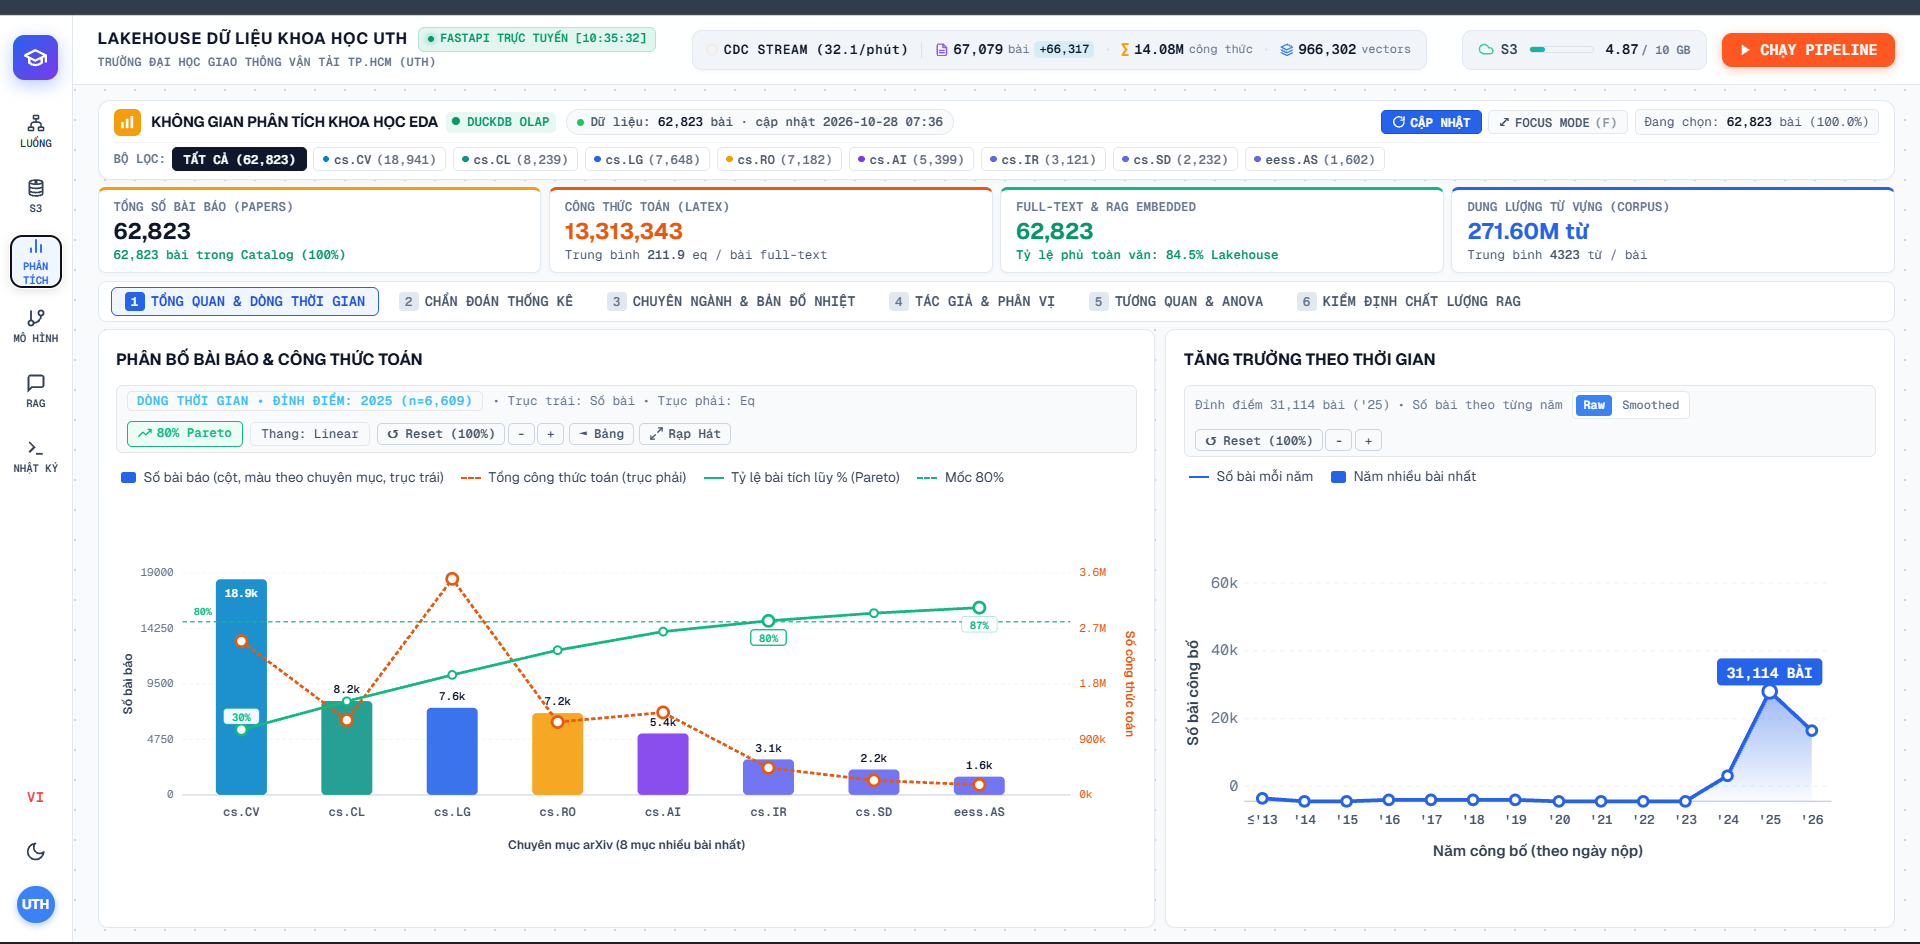
\includegraphics[width=\textwidth]{figures/eda_pareto_growth.png}
  \caption[Giao diện phân tích EDA (ảnh tư liệu)]{Giao diện phân tích EDA (ảnh tư liệu)}
  \ReportNote{Nguồn: ảnh lưu trong dự án LaTeX ngày 28/10/2026. Đây là giao diện của bản trước; số liệu trên ảnh không được dùng làm phép đo hiện tại.}
  \label{fig:eda_pareto_growth}
\end{figure}

\section{Các Phát Hiện EDA Cốt Lõi (Core Domain Insights)}

Quá trình khám phá dữ liệu thực nghiệm (EDA) kết hợp truy vấn cột DuckDB đã phát hiện những hiểu biết sâu sắc (insights) có ý nghĩa quyết định đối với việc thiết kế hệ thống khai phá và truy xuất RAG:

\subsection{Insight 1: "Đế chế toán học" tập trung ở \texttt{cs.LG} và \texttt{stat.ML}}
Số liệu Bảng~\ref{tab:eda_categories} cho thấy sự bất đối xứng rất lớn về hàm lượng toán học giữa các chuyên ngành:
\begin{itemize}
  \item Xét về \textbf{tổng số lượng công thức}: Chuyên ngành Học máy (\texttt{cs.LG}) chiếm vị trí thống trị tuyệt đối với \textbf{886,955 công thức toán} (chiếm tới gần 40\% toàn bộ công thức toán của cả kho dữ liệu). Mặc dù \texttt{cs.LG} và \texttt{cs.CV} có số bài xấp xỉ nhau (~2,300 bài), nhưng lượng công thức toán của \texttt{cs.LG} lại cao gấp \textbf{2.87 lần} so với \texttt{cs.CV}.
  \item Xét về \textbf{mật độ toán học trên từng bài báo (Mathematical Density)}: Chuyên ngành Thống kê Học máy (\texttt{stat.ML}) mới thực sự là "ông vua lý thuyết". Trung bình mỗi bài báo \texttt{stat.ML} chứa tới \textbf{669.9 công thức toán}, cao gấp 1.8 lần so với \texttt{cs.LG} (372.7 công thức/bài), cao gấp 5.0 lần so với \texttt{cs.CV} (135.8 công thức/bài), và gấp khoảng 6.6 lần so với chuyên ngành Xử lý ngôn ngữ tự nhiên \texttt{cs.CL} (102.2 công thức/bài).
\end{itemize}

\begin{calloutbox}{Ý nghĩa đối với thiết kế hệ thống}
Các khác biệt về mật độ toán học gợi ý cần đánh giá việc cắt đoạn theo cấu trúc học thuật. Code hiện phân đoạn theo section, cân bằng cửa sổ và ưu tiên ranh giới câu; chưa có cơ chế xác nhận mọi phương trình được giữ nguyên trong một chunk.
\end{calloutbox}

\subsection{Insight 2: \texttt{cs.AI} đóng vai trò "Trạm Trung chuyển Liên ngành" (Interdisciplinary Hub)}
Một hiện tượng bất ngờ là chuyên ngành Trí tuệ Nhân tạo (\texttt{cs.AI}) chỉ đứng thứ 5 về số lượng bài báo đơn lẻ (453 bài, chiếm 4.53\% dữ liệu). Tuy nhiên, khi phân tích ma trận đồng xuất bản (\textbf{Co-occurrence Matrix}), nhãn \texttt{cs.AI} lại xuất hiện trong hầu hết các cặp liên ngành lớn nhất:
\begin{itemize}
  \item $\texttt{cs.AI} \times \texttt{cs.LG}$: \textbf{1,521 bài} (Cặp lớn nhất trong artifact snapshot).
  \item $\texttt{cs.AI} \times \texttt{cs.CL}$: \textbf{786 bài} (Giao thoa giữa AI tổng quát và Ngôn ngữ học tính toán).
  \item $\texttt{cs.CV} \times \texttt{cs.LG}$: \textbf{732 bài} (Thị giác máy tính kết hợp các kỹ thuật Học sâu).
  \item $\texttt{cs.AI} \times \texttt{cs.CV}$: \textbf{615 bài} (Hướng tiếp cận Đa phương thức - Multimodal AI).
\end{itemize}
\textit{Ý nghĩa thực tiễn}: Trong snapshot được phân tích, các tác giả hiếm khi xuất bản một bài báo thuần túy dán nhãn \texttt{cs.AI}. Nhãn \texttt{cs.AI} hoạt động như một "siêu nhãn" (umbrella tag) bao bọc các nghiên cứu ứng dụng thực nghiệm vào Thị giác (\texttt{cs.CV}) hoặc Ngôn ngữ (\texttt{cs.CL}). Đây là cơ sở khoa học để xây dựng luật kết hợp mở rộng truy vấn trong Trụ cột 1.

\subsection{Insight 3: Độ lệch thời gian trong snapshot thu thập}
Artifact ghi 5,021 bài tháng 01/2024 và 3,797 bài tháng 02/2024, tổng 8,818 bài ($88.18\%$ của 10,000 bài). Phân bố này phản ánh phạm vi đợt thu thập; không đủ để suy luận tốc độ tăng trưởng của toàn bộ nghiên cứu AI/DS hoặc quy kết nguyên nhân cho Generative AI.

\subsection{Insight 4: Phân bố 4 góc phần tư giữa Mật độ Toán học và Độ dài Từ vựng}
Khi vẽ biểu đồ phân tán 2D giữa Số lượng từ vựng ($X \in [0, 12000]$) và Số lượng công thức toán ($Y \in [0, 1200]$), có thể dùng bốn vùng sau làm khung diễn giải định tính; artifact tổng hợp không xác nhận từng nhóm hoặc quan hệ nhân quả:
\begin{itemize}
  \item \textbf{Góc Q1 (Toán dày, Độ dài ngắn - Theoretical Rigor)}: Tập trung các bài báo \texttt{stat.ML} và \texttt{cs.LG} thuần lý thuyết, chứa nhiều chứng minh hội tụ và bổ đề giải tích.
  \item \textbf{Góc Q2 (Toán dày, Độ dài lớn - Foundational Monographs)}: Các công trình nghiên cứu quy mô lớn, luận án hoặc chuyên khảo nền tảng kết hợp cả lý thuyết sâu lẫn thực nghiệm rộng.
  \item \textbf{Góc Q3 (Toán ít, Độ dài ngắn - Short Communications)}: Các bài báo truyền thông hội nghị ngắn mô tả một phát hiện hoặc ứng dụng hẹp.
  \item \textbf{Góc Q4 (Toán ít, Độ dài lớn - Empirical Systems \& Benchmarks)}: Tập trung chủ yếu các bài báo \texttt{cs.CL} và hệ thống LLMs, chủ yếu trình bày kiến trúc, phân tích bảng kết quả thực nghiệm và ablation study dài hàng chục trang.
\end{itemize}


\section{Phân Tích Tương Quan Pearson và Spearman}
\label{sec:correlations}
Module \path{src/mining/eda_engine.py} có tính ma trận tương quan cho sáu thuộc tính của tài liệu toàn văn: số từ, số công thức, số mục, số tác giả, mật độ công thức trên 1,000 từ và số lượt trích dẫn. Mẫu phân tích lấy từ \texttt{fulltext\_view}, với số từ không rỗng và ít nhất 300. Mật độ toán được tính bằng số công thức chia cho $\max(\text{số từ},100)/1000$; lượt trích dẫn thiếu được điền bằng 0 theo code.

Pearson mô tả mức độ liên hệ tuyến tính; Spearman là tương quan Pearson giữa thứ hạng của hai biến, dùng để khảo sát quan hệ đơn điệu:
\begin{equation}
 r_{XY}=\frac{\operatorname{cov}(X,Y)}{s_Xs_Y},
 \qquad \rho_{XY}=r_{\operatorname{rank}(X),\operatorname{rank}(Y)}.
\end{equation}
Hệ thống gọi \texttt{scipy.stats.pearsonr} và \texttt{scipy.stats.spearmanr}, trả hệ số, p-value định dạng, ký hiệu mức ý nghĩa và cỡ mẫu; giao diện cho phép chuyển giữa hai ma trận. Vì vậy đây là chức năng đã có, không phải hạng mục triển khai trong tương lai.

Snapshot local được dùng trong báo cáo chưa có kết quả ma trận tương ứng để kiểm chứng. Báo cáo chỉ mô tả phương pháp, không bổ sung hệ số hoặc p-value thực nghiệm mới. Khi diễn giải cần lưu ý biến hằng, dữ liệu thiếu được điền 0, nhiều phép so sánh chưa hiệu chỉnh và thiên lệch thu thập; tương quan không chứng minh quan hệ nhân quả. Một số lời diễn giải trong code là chuỗi mô tả cố định, nên cần đối chiếu hệ số thực tế trước khi dùng làm kết luận.

\section{Vấn đề Chất lượng Dữ liệu và Giải Pháp Xử Lý}

Trong quá trình thu thập và tiền xử lý, hệ thống đối mặt với ba thách thức lớn về chất lượng dữ liệu:
\begin{enumerate}[label=\textbf{\arabic*.}]
  \item \textbf{Mất liên kết LaTeX do lỗi phân tích cú pháp}: Nhiều công thức toán học bị công cụ parse thông thường chuyển thành các ký tự rác. Hệ thống giải quyết bằng cách viết riêng module \texttt{AcademicHTMLParser} dựa trên \texttt{BeautifulSoup} và \texttt{lxml}, ưu tiên bóc tách từ thẻ \path{annotation encoding="application/x-tex"} để giữ LaTeX khi có dữ liệu nguồn phù hợp; chưa có kiểm định bảo toàn tuyệt đối trên toàn tập.
  \item \textbf{Trùng lặp tài liệu}: Fetch kiểm tra mã bài đã chuẩn hóa và hash abstract trong Silver. Khi compact papers, các bản ghi cùng \texttt{paper\_id} được gộp theo cơ chế last-write-wins; đây không phải quy tắc luôn chọn phiên bản nhiều từ/công thức nhất.
  \item \textbf{Độ lệch thời gian dồn cục (Collection Spike)}: Hiện tượng tập trung dữ liệu vào tháng 01/2024 do đặc thù đợt cào dữ liệu được nhận diện rõ ràng trong báo cáo nhằm tránh suy diễn sai lệch về xu hướng lịch sử dài hạn.
\end{enumerate}
